\documentclass{scrartcl}
\usepackage{amsmath}
\usepackage{hyperref}
\usepackage{color}
\usepackage{todonotes}
\usepackage{pdfpages}
\usepackage{subcaption}
\usepackage{minted}
\newcommand{\question}[1]{\todo[inline, color=blue!40]{#1}}
\newcommand{\note}[1]{\todo[inline, color=yellow!40]{#1}}
\newcommand{\means}{$\rightarrow{}$}

\begin{document}


\section{ToDos}
\begin{itemize}
    \item describe Ohua
    \item describe the actual problem
    \item are there other compilation approaches 
    \begin{enumerate}
        \item from any monolithic something to microkernel 
        \item from imperative lang to message passing 
        \item from dependent code to separation of concerns
    \end{enumerate}
    \item Linear State Usage/Transformation \means Do literature search!
    \item motivation: use notes\_motivation.md
\end{itemize}

\section{Notes on Papers -- 'Warehouse for Writing'}
\subsection{Unikernels}
\textbf{Unikernels: The Rise of the Virtual Library Operating System}
\begin{itemize}
    \item call 'operating systems virtualization' (Xen, VMWare) the key enabler of cloud computing
    \item downside: yet another layer on the software stack (e.g support for old physical protocols; irrelevant optimizations; backward-compatible interfaces (for example, Posix); user-space processes and threads (in addition to VMs on a hypervisor); and managed-code run-times (for example, OCaml, .NET, or Java). )
    \item Solution/Approach: MirageOS \means Compile single-purpose appliances 
    \begin{itemize}
        \item in style of a library operating system
        \item all code (HW interfacing, Hypervisor, OS kernel, user process, threads, language run-time, application code, configs) in the same language framework \means compiled to contain only necessary parts
        \item improves performance, reduces attack surface
    \end{itemize}
    \item hypervisors: horizontal scaling \means more cores/memory for a VM, vertical scaling \means more VMs
    \item external load balancers needed to spawn new VMs on load spikes, 
    \item 'traditional  OSes' 
    \begin{itemize}
        \item are not optimized for boot time and size (Windows system updates on boot \means you better keep booted idle machines for sudden spikes)
        \item are general purpose and have to handle diverse resources themselves 
        \item[]\means this is not the case for server appliances, where the hypervisor cares for resources and the requirements are 'single purpose application'
    \end{itemize}
    \item Problem: Existing Software relies on OS/System interfaces (POSIX, file system, network stack) to be present 
    \item \textbf{Library Operating Systems}:
    \begin{itemize}
        \item first were Exokernel and Nemesis10 in the late 1990s
        \item OS functions are implemented as libraries, protection boundaries are 'moved to the lowest hardware layers' \todo[inline]{clarify what that exactly means},
        \item policies implement access rights for applications using those libraries
        \item[]\means improves (predictability of) performance as applications access the HW resources directly i.e. not kernel-user-space switching 
        \item downsides: 1. running multiple applications side-by-side is tricky as resource access needs to be isolated, 2. device drivers need to be rewritten \means infeasible with fast evolving commodity hardware    
    \end{itemize}
    \item[] \means luckily these downsides \textbf{do not exists when hardware is abstracted by a hypervisor} i.e. for VMs
    \item \textbf{Typing, Memory Management, Modulization}: (re)writing kernels in high-level languages (other than C) provides the chance to avoid memory management, pointer and overflow bugs by language design (e.g. through strongly typed languages, static type checking, automatic memory management,  bounds checking, ...), for instance in ML (and we've just seen in Haskell) typing can also be used to enforce capability style access control \means even for the whole system if it's all based on one language run-time, further module systems i.e. support for encapsulation, separation of concerns 
    \item[]\means\textbf{Metaprogramming}: details of deployment/run-time system can be included in the code for static analysis and optimization via the compiler
    
    
    \item \textbf{MirageOS}: 
    \begin{itemize}
        \item based on OCaml, emits unikernels that run on Xen hypervisor
        \item compiler sees all dependencies including kernel libs as source code
        \item SAT solver is used to track module compatibility between user code and kernel libraries
        \item emitted code is a single-purpose Library Operating System VM (even bootloader is just a linked library), VM relies on hypervisor
        \item OCaml is used because a) static, strong typing b) supports functional, imperative and object oriented prgrmg and c) has a single-threaded run-time
        \item OCamls module system also features \textbf{parameterized module structures}, i.e. similar to header files in C but allowing type parameters \means provide module functors
        \item SAT solve approach allows \textbf{gradual recompilation} i.e. programmer can gradually replace kernel function by libraries, SAT solver will check, what is still needed from the monolithic kernel
        \item further backends \textbf{FreeBSD kernel module back end, JavaScript target by using the js\_of\_ocaml compiler}
        \item MirageOS libraries provide \textbf{serializable, explicite state handles}, \textbf{tree structured configuration is used to generate (metaprogramming) structure of the final appliance and initial state of the libraries }, similarly metaprogramming is used to generate a 'file system module' serving the needs of user code that only uses some files
        \item[]metaprogramming \means parts of the 'generating code' are not present in the 'generated code' \means compiled appliances can not just be repurposed without relinking or recompliation.
        \item ''In MirageOS, the OCaml compiler receives the source code for an entire kernel’s worth of code and links it into a stand-alone native-code object file. It is linked against a minimal runtime that provides boot support and the garbage collector. There is no preemptive threading, and the kernel is event driven via an I/O loop that polls Xen devices.''
        \todo[inline]{I don't fully get the life cycle description i.e. normal applications \means compiled to binaries \means be loaded into an OS process to run \means check configuration to tailor itself to the environment, many programs will use the same binary but with different config files}
    \end{itemize}
    \item \textbf{HalVM} similar to MirageOS, but in Haskell
    \item \textbf{ Drawbridge project } converts Windows into a libOS 
    \todo[inline]{Check out how Drawbridge does this? Might be a hint for our necessary code restructuring}    
\end{itemize}


\section{Open Questions}
\section{Thoughts and Ideas}
Use in general explanation and reasoning
\begin{itemize}
    \item domain knowledge of the programmer is expressed by choosing the scope and explicitly composing things she wants to be components later
    \item also actually the software already has to be written in message-passing style at least as long as we don't implement conversion of function calls to message formats
\end{itemize}
\begin{itemize}
    \item Do we need a similar approach as in MirageOS where libraries are linked to the application by initializing their (serializable) state handle?
    \item How does the level of separation of concerns in unikernel relate to our microkernel target? 
    \begin{itemize}
        \item '' rather than treating the database, Web server, and so on, as independent applications that must be connected by configuration files, they are treated as libraries within a single application,'' \means the idea of compiling a composition in the host language is pretty similar
        \item libraries have their own state \means this looks like basically connecting stateful functions
        \item both argument via a) static type checking b) simple composition c) eliminating config files
        \item not sure what they mean by 'flipping the switch' but they point out the ability to build and test as usual Unix applications and then 'flip the switch' and deploy as single purpose VMs 
        \item when they talk about \textit{single-purpose} they seem to talk about one application with all required code e.g. network stack, db stuff  to run it \means we talk about separating this further, horizontally i.e. separate  NIC interface from TCP/IP from Application  so unikernel \means microkernel 
        \item They talk about pressure imposed on the hypervisor. How does this work out for us? Who manages processes (and VMs) at what level of separation?
    \end{itemize}
    \item Related/terms: WPO (Whole Program Optimizer, 'pioneer' MLton) \means in case of libOSes 'whole program' includes the OS
    \item How does security of container, the unikernel/libOS approach and the microkernel approacch relate?...And why?
    \item Related Work ? : Generating Packet parsing Code and integrating it with smolTCP \cite{GenerateCode}
    \item Designing Systems: One argument for microkernels Carsten mentions (and actually it really follows from the principle) is, that they enforce compartmentalization i.e. make the programmers structure their application from independent components and have only explicit communication relations (no sharing things). How do we think about this argument in our approach. Clearly, composition is the way to structure things in our approach, but do we enforce the same strictness of isolation and more over ...
    \item What if libraries (i.e. code we don't look at) entail function calls and shared data among later separated components?
\end{itemize}

\section{Remaining notes on Rust}
\note{Note to myself: Allocation only refers to heap memory}
\note{Say something about deref coercion? Probably not }
\textbf{Closures}: Closures are used in smotcp quite a lot so its important to understand how this influences state sharing and control flow in the original architecture.
\begin{itemize}
    \item if not explicitly annotated, the closure will derive if captured objects are mut/immut borrowed or moved 
\end{itemize}
\begin{minted}{rust}
let obj1 = OBJ1::new();
let closure1 = |arg| {let x =obj1.do_stuff(arg);
                      x*2}
// closure1 is moved to use_closure, 
// while obj2 gets a mutable reference to obj1
obj2.use_closure(closure1);
\end{minted}


Features of Rust that might become relevant for implementation
\begin{itemize}
    \item Type Inference: Rusts type inference is based on standard Hindley-Milner (HM) type inference algorithm\footnote{Full description can be found in \href{https://rustc-dev-guide.rust-lang.org/about-this-guide.html}{the Guide to Rustc Development}}. To resolve trait bounds a Unification algorithm similar to the algorithm used in Prolog to solve logical constraints\footnote{The Trait Bound Unification is implemented in the \href{https://rust-lang.github.io/chalk/book/}{Chalk} library}.
    \todo[inline]{If needed and time allows check (reasons for) limitations and give details on extensions}
    \item Generic Types: To allow the use of generic types with basically no runtime overhead, Rust uses so called \textit{monomorphization} at compile time. This process infers concrete typing for any use of generically typed elements, like functions, structs or enums. The concretely typed instances of elements are then inlined to the existing code. It is in fact one of the last steps on a Rust IR before the code is lowered to LLVM IR and passed to LLVM for code generation and enables LLVM to infer some lower level optimizations (city rustc guide again? ).
    \item Serialization: There is a crate \href{https://doc.rust-lang.org/nightly/nightly-rustc/rustc_serialize/index.html}{serialize}, that as described in the 
\end{itemize}

\todo[inline]{Tail recursion support is limited in Rust, meaning the compiler is able to derive tail call elimination in simple cases but is not guaranteed to do so.}
\subsection{Fragments left for reuse/disposal}
%In fact, there are two main aspects that need to be considered. The first is, that we need to present the compiler our target components and their basic interaction as stateful objects in the compile scope. It must be recognizable for the compiler, what the stateful components of the program are and how they interact. In particular, we must not as smoltcp currently does, give the device as a parameter to the TCP/IP component and let the later use the device 'under the hood', i.e. inside the library and outside the compile scope. The second aspect is, that all communication between components must be done explicitly via serializable messages, not via access to shared memory as before.

%The first, and most trivial change is encapsulating initialization into \rust{init_<component>()} functions. This also entails encapsulating the sockets and the interface from the original code into one component.
%\todo[inline]{refactor example and add description when I know how I handle the socket handles}

%Second we notice that each of our components is used only once in our target program. The function \rust{poll} that contains the interaction of  TCP/IP stack and the device to receive and send messages must become a pure function, i.e. taking both the TCP/IP stack and the device as arguments. We must lift it into compile scope and refactor the  usage of both components in the function to also follow our programming model. To enable this linear usage of states, we obviously need to transform the way those stateful components work in smoltcp. In Section~\ref{subsec:StateThreading} we further illustrate the problem and explain how to approach it.

%Thirdly we see, that the communication between the components does not happen through mutual access to states anymore. For example, instead of accessing a socket directly via \rust{let socket = sockets.get_mut::<tcp::Socket>(tcp_handle);} we need to implement a data format and a command interface in both the \rust{app} component and the \rust{tcp_ip_stack} to enable such interactions via message passing. We discuss this issue in Section~\ref{subsec:MessagePassing} and present our implementation as a possible solution.

%Finally we have to use a recursion instead of a \rust{while} loop. This is a current restriction of Ohua which we discuss in more detail in Section~\ref{subsubsec:WhileLoops}. 
%\note{Note to me: Ohua also supports 'endless' for loops. However we have no way of gracefully ending them as we a) can not access the loop generator while running and b) we do not support early returns i.e. \rust{break} or \rust{return}}
%\todo[inline]{figure out recursion}

Those todos where left from RW. I didn't manage to read them but htey might be interesting.
\todo[inline]{ Check \cite{9973038}: Combined approach using HW protection techniques, compile time analysis, model checking, and compiler runtime measures for protection. Probably cites a lot of approaches.}

\todo[inline]{ Abraham A Clements, Naif Saleh Almakhdhub, Saurabh Bagchi, and Mathias
Payer. ACES: Automatic compartments for embedded systems. In 27th USENIX
Security Symposium (USENIX Security 18), pages 65--82, Baltimore, MD, Au-
gust 2018. USENIX Association.
}

Paper Stack Notes - Just for me now
\begin{itemize}
    \item Language-Agnostic Optimization and Parallelization for Interpreted Languages \means interesting is, that they don't use the language itself but analyze (static+dynamic) traces from the respective interpreters (with all problems that implies as having to separate interpreter introduced flow/dependencies from code flow/dependencies), they derive (or propose to do so) parallelity on the LLVM IR level
    \item Definitional Interpreters for Higher-Order Programming Languages \means very interesting for basic ideas (and wtf is GEDANKEN? Is it an actual language?), but for now to far off
    \item Software Compilation Techniques for
Heterogeneous Embedded Multi-Core Systems \means paper from our chair (at east Jeronimo is on the author list), point is that compilers for MPSoC should except sequential code for the same reasons we bring forward, same time the backend has to distribute parallel tasks in a more coarse grained fashion than single-core compilers do (ILP) \means maybe, if we come to the conclusion that atuomatic extraction of components is possible and stateful components should be annotated, why not annotate them with target architecture directive \means anyway that's just a (faaaarrrr) outlook perspective
\end{itemize}

\todo[inline]{ I don't know where to put this so I don't forget, Danvys Dr.Sc. Thesis is titled "An Analytical Approach to Programs as Data Objects". Given the chapter titles I think its quite interesting and might be a good start to get the background for transformations}
\section{remains from related work}
The general idea to transform programs into data flow automatically is wide spread in particular in data processing and web applications. In case of Big Data applications it is mostly the sheer size of states as for example a trained model that makes 
state transfer impossible, in case of web applications and client server interactions the interesting question is rather which parts of the server execution state should be stored or send to the client in order to serve multiple clients in an asynchronous fashion.

Here we will only look at some examples for data flow graph compilation, because they illustrate common problems. For example in \cite{fernandez2014making} the goal here was to support arbitrary stateful Java objects in Big Data applications and to recover states upon failures. They distinguish types of state access 

\begin{itemize}
    \item approach: infer dataflow and 'types of state access' to derive a 'stateful dataflow graph'(SDG)
    \item they explicitly focus on 'large states', where distribution of such state to several nodes is desirable both for performance/(storage/compute) capacity and for recovery after failure 
    \item SGD: "cyclic graph of pipelined data-parallel tasks, which execute on different nodes and access local in-memory state" \means no explicit scheduling
\item to identify 'partial' and 'partitioned' stateful objects, they require annotations from the programmer
\item they describe some concepts for parallel state handling and failure recovery, which might be helpful later
\item Graph derivation itself is not to fancy/smart \means  they require different annotations from the programmer to identify how particular states should be used (e.g. if they are global, mutable, can be partitioned etc), 
\item Limitiations:
\begin{itemize}
    \item programmer needs to annotate how states are used
    \item programmers need to implement the required primitives to handle state in the graph themselves (serialization, definitions for partitioning and recovery) or use predefined classes
    \item no side-effects on 'single valued' terms (marked by programmer), e.g. used as arguments for (stateful) computations
    \item deterministic execution: that's basically a requirement for sem. correct failure recovery e.g. program should not depend on current time or similar external state 
\end{itemize}
\item We do not aim to distribute the state handling itself, otherwise limitations/prerequisites are pretty similar
\item they work with checkpoints for failure recovery and synchronization of states and node replication (also for stateful nodes) to eliminate runtime bottlenecks \means not relevant for now, maybe later
\end{itemize}

Another example is the DFGenTool~\cite{mukherjee2017dfgentool}. It generates a graph representation (DFG in DOT format) from a given program in LLVM IR. This has several advantages for the tool. Using LLVM it is language independent to a certain degree. The LLVM IR also has features that make graph derivation much easier. In particular, during compilation to this IR, conversion to SSA format, simplification of instructions and division of the control flow into basic blocks have already been performed. It is also ensured that values are only used once and that copies are generated for values that enter a divergent control flow. To extract the actual stateful components as well as to distinguish handling mechanisms for states are used read only vs. states that need 

\begin{itemize}
    \item 
\means advantages are obv. language+backend independence, but also that Basic Blocks are already identified and separated easing the conversion to nodes.
    \item available, though not maintained at \url{http://github.com/manideepam/DFGenTool}
    \item LLVM already provides SSA form, the guarantee that values are used only once and that copies are produced for values entering diverging control flow, also supported data types, by the looks of it are only int, float and arrays. Also to handle reassignments load and store dependencies are derived using LLVM alias analysis module
    \item \means maybe another example for easier scenarios but not helpful to get ahead, I might check how LLVM alias analysis module works though
\end{itemize}

"Automatic Extraction of Coarse-Grained Data Flow Threads from Imperative Programs" 
\begin{itemize}
    \item prototype compiler based on GCC for rec. C code
    \item only pure functions
    \item works on SSA representation
    \item interesting part: building program dependency graph from SSA (PDG), fuse strongly connected components (SCCs) using dependency analysis (simplified, eg. no arrays) \means "typed fusion", aligning dependency and data flow to data-flow-program-dependency-graph DF-PDG \means conversion algorithms     
    \item interesting also: mentions decoupled software pipelining (DSWP) technique \means Is it relevant for us?
\end{itemize}


\textbf{Cooperative Task Management without Manual Stack Management
or, Event-driven Programming is Not the Opposite of Threaded Programming}~\cite{adya2002cooperative}
\means I think they also describe the transformations we are looking at, at least the part after components are inlined  but they explain it as a process from automatic to manual stack management
\begin{itemize}
    \item they bring some arguments and nice explanations for different concepts in
    concurrent programming in particular event-driven (cooperative tasks) vs. multi-threaded (preemtive or serial task management)
    \item event-driven is (according to the authors) easier to reason about concerning concurrent correctness
    \item the rest of the paper explains how both types of stack management can be/are used together using cooperative scheduling in Windows (using threads and fibers respectively)
\end{itemize}


\textbf{Continuations from Generalized Stack Inspection}\cite{}
\begin{itemize}
    \item a problem not addressed in CPS is the preservation of the run-time stack for "decomposed" functions
    \item there are languages like Scheme, that provide first-class continuations (i.e. they can be entirely send around) but most languages (in particular those running on VMs) do not provide means to programmatically save and reinstate the run-time stack. 
    \item One Solution was to move the run-time stack to the heap (there's just a sourceforge link in the bibliography :-( ), which is effectively what we did.
    \item The authors use a mechanism called \emph{continuation marks}. They are a form of stack inspection, enabling the programmer to attach values to the control flow stack and set marks, indexed by keys to the stack to later retrieve those values. In a first step they transform a Scheme program into this representation, in the second they use the marks to derive defunctionalization
    \item \means Not sure but this looks like deciding to integrate intermediate values into the data flow, while we decided to make them part of the local heap of stateful objects.
\end{itemize}
\todo[inline]{Check HAKC\cite{mckee2022preventing}, Endokernel\cite{im2021endokernel}}

\section{"Workflow" for Automatic transformation}
Remaining notes and question for 'automatization'
\begin{itemize}
    \item to support lambda lifting this way, a language needs to support sum type definition i.e.
    \code{type Functions = DoThis | DoThat | DoSomethingElse}
    Further difficulty: What traits do we need to derive? Obviously Clone and that needs to work because \means all arguments need to implement Clone. What else? Can we assume or derive automatically? 
    \item Bound variables, i.e. direct function arguments are just included in the function data types (as far as the language supports this, otherwise the Function type needs to represent any possible value of the arguments as individual type). In case of Rust, this is not a problem as sum types can be defined as \rust{enum}s which support additional data
    \item Free Variables, i.e. enclosed values from functions that where closures usually require lambda lifting. The term basically already describes the underlying principle, namely that free variables in a function are \emph{lifted} to the definition of the function as parameters i.e. bound by the lambda expression defining the function and the function itself is \emph{lifted} to a global scope. A simple example is shown in Figure~\ref{fig:lambdaLift}.
    \item process \means identify a) basic blocks b) data dependencies \means define function data types, arguments to constructors are data from other components \means define \rust{apply} function \means pattern matching on enums, code in match arms is code called directly before, if we were inside a state before, we need to retrieve and set the state to restore the behavior of the original 'closure'/subcall \means replace jumps and calls to other component with return \means overall return is union of original return and calls to other components
    \item If arguments follow the control flow they become part of the data type definition for the functions
    \item If arguments do not follow the control flow, i.e. if they belong to only one component, they are made part of the components state. This is particularly the case for the socket being processed in each round.
    \item particular issue occurring are lifetimes and ownership. Regardless whether we send values, or store them inside the state they must not reference each other. This is because we split a function, in this case \stack{.socket_egress} and thereby distribute execution that ran on one stack frame to multiple stack frames. As explained in the Background Section~\ref{subsec:Rust} this means that references, bound on the stack frame of one sub-function, can become invalid when the function exits and cannot just be stored in the \stack{}s state for usage in the next sub-function. This becomes particularly obvious when we look at the loop over the sockets. 
    \item In the sequential program four references to the same object exist simultaneously i) the sockets, ii) the iterator on the sockets iii) the current socket and iv) the packet, which internally holds a reference to the sockets memory. 
\end{itemize}

\section{Remaining transformation notes}



Enable stateful computation in branches. Figure~\ref{fig:DFBranching} shows, how branching and stateful call are represented as dataflow graphs. A branching section is guarded by node evaluating the condition, this node produces three output signals. Two of them are control signals, the third one is the boolean evaluation result. The control signals are used by control nodes in the respective branch to guard the execution of the branch. In the \emph{active} branch, the control node will receive the first input and send the first intermediate result for the branch. In our example there is just one input and result per branch, so actually the control nodes and the function nodes \rust{f(x)} or \rust{g(x)} are fused. Finally a \textbf{select} node receives the evaluation result and based on this result decides on which channel to receive the next result from. In our example, if the evaluation resulted in \rust{a = true}, the \rust{select} node tries to receive from the \rust{r1} channel. As receiving is blocking, this ensures that results are received in the same order as the branching instructions where send and therefore that determinism is preserved even if branches act independently.  
\begin{itemize}
    \item we also see how stateful operations are translated
    \item so first 'issue' to integrate stateful ops in branching is, that we need to thread a tuple of \rust{(obj, result)} instead of just the result
    \item another problem is obv. concurrency. When branches are pure, one branch can start, while the other one is still busy. How can we ensure, that the correct operation uses the correct 'incarnation' of the object, if an object is used in both branches?
    \item Case 1: Object used only in one branch
    \item Case 2: Object is used in both branches
    \item Case 3: Objcet is used more than once.
\end{itemize}
\begin{figure}[H]
\centering
\tabskip=0pt
\valign{#\cr
    \hbox{%
    \begin{subfigure}{.25\textwidth}
    \centering
     \begin{minted}[fontsize=\footnotesize]{rust}
    if a {
        f(x)
    } else {
        g(x)
    }
     \end{minted}
    \end{subfigure}
    \begin{subfigure}{.72\textwidth}
    \centering
    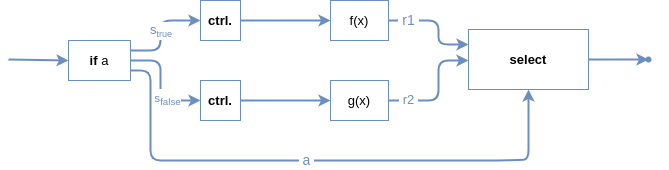
\includegraphics[height=3cm]{figures/branching_ohua.png}
     \label{subfig:branchingGraph}
    \end{subfigure}%
  }
  \cr
  \noalign{\hfill}
    \hbox{%
    \begin{subfigure}{.25\textwidth}
    \centering
     \begin{minted}[fontsize=\footnotesize]{rust}

     obj.do(x)

     \end{minted}
    \end{subfigure}    
    \begin{subfigure}{.72\textwidth}
    \centering
    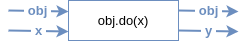
\includegraphics[height=1cm]{figures/method_ohua.png}
     \label{subfig:methodGraph}
    \end{subfigure}%
  }
  \cr
}
\caption{}
\label{fig:DFBranching}
\end{figure}
\todo[inline]{Check where the below comments belong}
\note{Finally there are some open question we need to address regarding accepted types. Currently the type extraction mechanism just wraps any relevant type annotation from the input code in a to an internal argument type representation. This means, we do not distinguish the actual Rust types and do not filter for references, pointer or trait objects. The goal is of course to develop Ohua and the programming model for Rust to the point where a valid sequential input program never leads to an invalid output program, i.e. we want to achieve soundness. For this we need to evaluate if and how the type system of Rust has to be restricted in the input. And so we need to decide whether to leave this to the programmer, because it depends for example on the chosen backend or if there have to be additional mechanisms in the compiler to enforce these restrictions. We might also need to extend the programming model by necessary augmentation on the original program, like additional trait bounds. For example, an automatic annotation with \rust{[\#derive]} could be generated to add traits, e.g. for serialization that were not necessary in the serial program. We will consider those question in the further development of Ohua and in particular the Rust integration.}


\end{document}
